%---------------------------------------------
%---------------------------------------------
%---------------------------------------------
%---------------------------------------------
\exercise{Robotics in a Nutshell}
You are considering to buy a new multi-purpose robot platform. Its kinematic chain has two rotational $q_{\{1,3\}}$ and two linear $q_{\{2,4\}}$ degrees of freedom (DoFs), as shown in the figure below. These four joints are actuated with forces and torques of $u_i$, $i\in\{1,2,3,4\}$. A gripper is mounted on the end of the robot, indicated by the letter \textbf{E}. The robot's base is mounted on a table. We assume that the base Cartesian coordinates at the mount are $x_\textrm{base}=[0,0,0]$.  

\begin{center}
   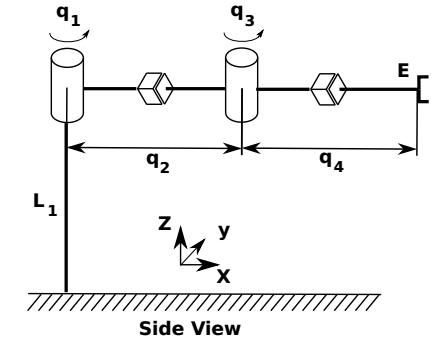
\includegraphics[width=0.35\textwidth]{img/robot.png} 
\end{center}



\begin{questions}

%----------------------------------------------

\begin{question}{Forward Kinematics}{2}
Compute the kinematic transformation in the global coordinate system from the base $\vec{x_\textrm{base}}$ to the end-effector \textbf{E}.  
Write the solution for the $\vec{x_\textrm{end-eff}}=[x,y,z]^T$  according to the joint values $q_i$, where $i \in \{1,2,3,4\}$.

\begin{answer}
	Compute the position with rotation and translation matrices:
	\begin{equation}
		\begin{split}
			H_5 &= Trans_{z,l1}\cdot Rot_{z,q_1}\cdot Trans_{x,q_2}\cdot Rot_{z,q_3}\cdot Trans_{x,q_4}\\
			H_5 &= 
			\begin{pmatrix} 
				1& 0& 0& 0\\
				0& 1& 0& 0\\
				0& 0& 1& L1\\
				0& 0& 0& 1
			\end{pmatrix}
			\cdot
			\begin{pmatrix}
				c_{q_1}& -s_{q_1}& 0& 0\\
				s_{q_1}& c_{q_1}& 0& 0\\
				0& 0& 1& 0&\\
				0& 0& 0& 1&
			\end{pmatrix}
			\cdot
			\begin{pmatrix} 
				1& 0& 0& q_2\\
				0& 1& 0& 0\\
				0& 0& 1& 0\\
				0& 0& 0& 1
			\end{pmatrix}
			\cdot
			\begin{pmatrix}
				c_{q_3}& -s_{q_3}& 0& 0\\
				s_{q_3}& c_{q_3}& 0& 0\\
				0& 0& 1& 0&\\
				0& 0& 0& 1&
			\end{pmatrix}
			\cdot
			\begin{pmatrix} 
				1& 0& 0& q_4\\
				0& 1& 0& 0\\
				0& 0& 1& 0\\
				0& 0& 0& 1
			\end{pmatrix}\\
	%        
			H_5 &= 
			\begin{pmatrix}
				\cos(q_1+q_3)& -\sin(q_1+q_3)& 0& q_4\cos(q_1+q_3) + q_2\cos(q_1)\\
				\sin(q_1+q_3)& cos(q_1+q_3)& 0& q_4\sin(q_1+q_3) + q_2\sin(q_1)\\
				0& 0& 1& L1\\
				0& 0& 0& 1
			\end{pmatrix}
		\end{split}
	\end{equation}
	
	So the position of the end-effector is: 
	\begin{equation}
		\begin{split}
			x_e &= q_4\cos(q_1+q_3) + q_2\cos(q_1)\\
			y_e &= q_4\sin(q_1+q_3) + q_2\sin(q_1)\\
			z_e &= L1
		\end{split}
	\end{equation}

	\end{answer}

\end{question}

%----------------------------------------------

\begin{question}{Inverse Kinematics}{2}
Define briefly in your own words the inverse kinematics problem in robotics.  
Can we always accurately model the inverse kinematics of a robot with a
function?

\begin{answer}
	Forward Kinematics: \\
	with the given angles $\vec{q}$ you calculate the $\vec{^0T_E} = \begin{bmatrix} ^0R_E & ^0r_E \\ 0^T &1\end{bmatrix}$ matrix. 
	
	Inverse Kinematics:\\
	with the given Pose (Orientation $\vec{^0R_E}$ and position $\vec{^0r_E}$) from the world coordinate system to the Endeffector coordinate system you can calculate the desired joint angles $\vec{q}$. The method therefore is called Inverse Kinematics (Inverse Euler or Inverse Roll Pitch Yaw method are possible.)\\
	
   The INV KIN cannot always be modeled accurately because:
   \begin{itemize}
   	\item if n<6  the INVKIN has no solution, $n=\sum_i \vec{q}_i$ 
   	\item if n=6  the INVKIN has one solution
   	\item if n>6  the INVKIN has infinity solutions (Redundancy)
   \end{itemize}

   The technical background of this is, that the robot can reach a end-effector position in task space with many different positions in joint space. So the inverse kinematics are not a function.

   Although you can build robots with only a few degrees of freedom which have clearly invertible kinematics. This is often done for industrial robots.
   
	

	\end{answer}

\end{question}

%----------------------------------------------

\begin{question}{Differential Kinematics}{4}
Compute the Jacobian matrix $\vec{J}(\vec{q})$ of the robot such that $\dot{\vec{x}}=\vec{J}(\vec{q})\dot{\vec{q}}$, where $\dot{\vec{q}}$ is the first time derivatives of the state vector $\vec{q}$ of the robot. Explain in a sentence the physical meaning of the Jacobian.

\begin{answer}
	Theory:\\
	$\vec{\dot{x}} = \vec{J(\vec{q})} \vec{\dot{q}}, \quad \begin{bmatrix}
	^0\vec{v}_n(t) \\ ^0\vec{\omega}_n(t)
	\end{bmatrix}= ^0\vec{J}_n(\vec{q}(t)) * \vec{\dot{q}}(t), \quad ^0J_n = \begin{bmatrix}
	^0J_{n,v}\\^0J_{n,\omega}
	\end{bmatrix}, \quad ^0J_n \in 6 x n \quad$$^0J_n = [^0J_{n,1}, ..., ^0J_{n,n}]$ (split into vectors)
	$\quad ^0\vec{R}_E=(^0\vec{e}_x,^0\vec{e}_y,^0\vec{e}_z)$
	\\
	
	
	There are basically 2 ways to calculate the Jacobian Matrix. \\
	\noindent\hspace*{20mm}1. Get the Jacobian with the $^0T_{i-1}$\\
	\noindent\hspace*{25mm} If $q_i = \Theta_i$ revolute joint:\\
	\noindent\hspace*{30mm} $^0J_{n,i} = \begin{bmatrix}
		^0e_{z,i-1} x (^0r_n - ^0r_{i-1}) \\ ^e_{z,i-1}
		\end{bmatrix}$\\
			\noindent\hspace*{25mm} If $q_i = \Theta_i$ prismatic joint:\\
			\noindent\hspace*{30mm} $^0J_{n,i} = \begin{bmatrix}
			^0e_{z,i-1} \\\vec{0}
			\end{bmatrix}$\\
		\noindent\hspace*{20mm}2. Get the Jacobian with the $^0T_{n}$\\		
		\noindent\hspace*{25mm} $^0v_n(t)=^0\vec{\dot{r}}_n(q(t)) \dot{R(q)}$\\
		\noindent\hspace*{25mm} $^0\omega_n(t): B(q(t),\dot{q(t)})=\frac{\partial R (q(t))}{\partial q(t)} * \dot{q(t)}* R^T(q(t)), \quad B = \begin{bmatrix}
		0 & -\omega_z &\omega_y \\ \omega_z & 0 & -\omega_x \\ -\omega_y &\omega_x&0
		\end{bmatrix}$\\
	Physical Meaning:\\
	
	\begin{equation}
		J = 
		\begin{pmatrix}
			-q_4\sin(q_1+q_3) - q_2\sin(q_1)& 
			\cos(q_1)& -q_4\sin(q_1+q_3)& \cos(q_1+q_3) \\
			q_4\cos(q_1+q_3)+q_2\cos(q_1)& 
			\sin(q_1)& q_4\cos(q_1+q_3)& \sin(q_1+q_3)\\
			0& 0& 0& 0&
		\end{pmatrix}
	\end{equation}
	
	The jacobian describes the relationship between the end-effector velocity an the velocity of the different joints.
	
	\end{answer}

\end{question}

%----------------------------------------------

\begin{question}{Singularities}{3}
What is the kinematic singularity in robotics? How can you detect it? When does our robotic arm, which was defined above, enter a kinematic singularity?

\begin{answer}
	Singularities occur if $det(^0\vec{J}_n(q))=0$. \\This can happen for instance if the rotational axis of two joints is the same in such a case one DOF is lost. So simply checkout if a certain row or column of the Jacobi matrix gets zero for special joint values. 
	
	To analyze the kinematic singularity of the robot, you only have to look at rotational joints. The translational joint cannot move into a singularity. So you can build a reduced jacobian:
	\begin{equation}
		J_{red} = 
		\begin{pmatrix}
			-q_4\sin(q_1+q_3) - q_2\sin(q_1)& -q_4\sin(q_1+q_3)\\
			q_4\cos(q_1+q_3)+q_2\cos(q_1)& q_4\cos(q_1+q_3)
		\end{pmatrix}
		\end{equation}
	
	In a singularity the determinat of $J_red$ equals zero. So we can calculate it and find the roots:
	
	\begin{equation}
		\det J_{red} = q_2 q_4 \sin(q_3)
	\end{equation}
	\begin{equation}
		\begin{split}
			\text{The roots are:}\\
			q_2 &= 0\\
			q_4 &= 0\\
			q_3 &= 0 \lor \pi
		\end{split}
	\end{equation}
	
	The robot hits singularities when the translational joints $q_2$ or $q_4$ are at the zeros position. Then the joints $q_1$ and $q_3$ are at the exactly same position in task space. However these singularities are never reached because of the technical limits of the robot. So the only important singularity is the third. The joints $q_2$ and $q_4$ are on the same axes and the robot loses one degree of freedom.
	
	\end{answer}

\end{question}

%----------------------------------------------

\begin{question}{Workspace}{1}
If your task is to sort items placed on a table, would you buy this robot? Briefly justify your answer.

\begin{answer}
	The robot can only reach positions with the coordinate $z=L1$. Because of this we would not buy the robot for this task.
\end{answer}

\end{question}

\end{questions}
